\documentclass[11pt, oneside]{article}   	% use "amsart" instead of "article" for AMSLaTeX format
\usepackage{geometry}                		% See geometry.pdf to learn the layout options. There are lots.
\geometry{letterpaper}                   		% ... or a4paper or a5paper or ... 
%\geometry{landscape}                		% Activate for for rotated page geometry
%\usepackage[parfill]{parskip}    		% Activate to begin paragraphs with an empty line rather than an indent
\usepackage{graphicx}				% Use pdf, png, jpg, or eps§ with pdflatex; use eps in DVI mode
								% TeX will automatically convert eps --> pdf in pdflatex		
\usepackage{amssymb}
\usepackage{amsmath}
\usepackage{parskip}
\usepackage{color}
\usepackage{hyperref}

\title{Writing a Laurent Series}
%\author{The Author}
%\section{}
%\subsection*{}
\date{}							% Activate to display a given date or no date

\graphicspath{{/Users/telliott_admin/Dropbox/Tex/png/}}
% \begin{center} 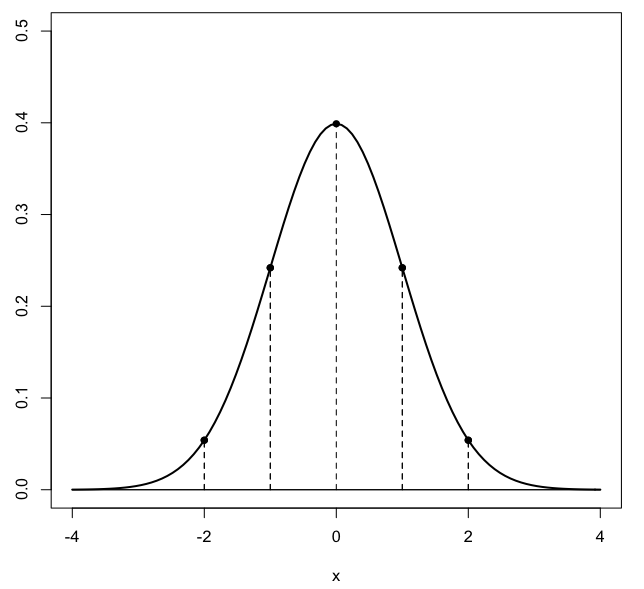
\includegraphics [scale=0.4] {gauss3.png} \end{center}
\begin{document}
\maketitle
\Large
\subsection*{example}
Suppose
\[ f(z) = \frac{z}{(z-1)(z-3)} \]
and say we need the series around $0 \le | z - 1 | \le 2$, a circle of radius $2$ around the point $z_0 = 1$.

One way is to do the substitution $x = z - 1$, so $z = x + 1$ and we have
\[  = \frac{x+1}{(x)(x-2)} \]
and then our goal is to get something like $1/1-x$.  Factor out the $1/x$
\[ = \frac{1}{x} \ ( \frac{x+1}{x-2} ) \]
Get $x - 2$ on top
\[ = \frac{1}{x} \ ( \frac{x - 2 +  3}{x - 2} ) \]
\[ = \frac{1}{x} \ ( 1 + \frac{ 3}{x-2} ) \]
\[ = \frac{1}{x} \ ( 1 - \frac{ 3}{2-x} ) \]
\[ = \frac{1}{x} \ ( 1 - \frac{ 3/2}{1 - x/2} ) \]
\[ = \frac{1}{x} \ ( 1 - \frac{3}{2} \cdot \frac{1}{1 - x/2} ) \]
and now the 
\[ \frac{1}{1 - x/2} \]
can be expanded because
\[ \frac{1}{1 - y} = 1 + y + y^2 + y^3 \]
so 
\[ \frac{1}{1 - x/2} = 1 + \frac{x}{2} + (\frac{x}{2} )^2 + \dots \]
which gives
\[ = \frac{1}{x} \ [ 1 - \frac{3}{2} \cdot (1 + \frac{x}{2} + (\frac{x}{2} )^2 + \dots) \ ] \]

Now, multiplying through by $1/x$ gives
\[ -\frac{1}{2x} + \dots \]
\[ = -\frac{1}{2(z-1)} + \dots \]
which we will integrate as
\[ \oint \frac{-1/2}{z-1} \ dz \]
\[ \text{Res }(1) = \lim_{z \rightarrow 1} (z-1) \ \frac{-1/2}{z-1} \]
\[ = -\frac{1}{2} \]
Multiply by $2 \pi i$ to obtain $I = \pi i$.

As a check on this go back to 
\[ f(z) = \frac{z}{(z-1)(z-3)} \]
\[ \text{Res }(1) = \lim_{z \rightarrow 1} (z-1) \ \frac{z}{(z-1)(z-3)} \]
\[ =  \lim_{z \rightarrow 1} \ \frac{z}{z-3} \]
\[ = -\frac{1}{2} \]

\subsection*{example}
These examples can get really complicated.  Here is one from

\url{http://zimmer.csufresno.edu/~doreendl/128.13f/handouts/Lseriesex.pdf}

Consider the very simple example:
\[ f(z) = \frac{1}{(z-2)(z-1)} \]

This function has poles at $z = 1$ and $z = 2$.  If we are asked to write expansions around $z_0 = 0$, then we have three regions of interest and three different expansions.

The first region is the circle of radius $1$:  $|z| < 1$, the second is $1 < |z| < 2$ and then finally $|z| > 2$.

\subsection*{region 1}
Use partial fractions to write:
\[ \frac{1}{(z-2)(z-1)} = \frac{1}{z-2} - \frac{1}{z-1} \]
Considering the second term, we bring the minus sign inside
\[ = \frac{1}{z-2} + \frac{1}{1-z} \]
We have the classic
\[ \frac{1}{1-z} = 1 + z + z^2 = \sum_{n=0}^{\infty} z^n \]
which we know this is valid for $|z| < 1$, the region of interest.

For the other term
\[ \frac{1}{z - 2} = - \frac{1}{2 - z} \]
Our goal is to convert this into something like the geometric series.  Factor out the $2$ on the bottom like so
\[ = - \frac{1}{2} \ [ \  \frac{1}{1 - z/2} \ ]  \]
We can do a formal substitution or recognize that this is the geometric series 
\[ = - \frac{1}{2} \ [ \   \sum_{n=0}^{\infty} (z/2)^n \ ]  \]
We can rewrite this slightly by pulling out the factor of $2^n$ on the bottom and combining it with the factor of $2$ out front:
\[ = \sum_{n=0}^{\infty} \ [ \ \frac{-1}{2^{n+1}} \ ] \  z^n \  \]
which converges for $0 < |z/2| < 1 \Rightarrow 0 < |z| < 2$.

Our series is the sum of these two series, which can be combined as
\[ \sum_{n=0}^{\infty} \ [ \ 1 - \frac{1}{2^{n+1}} \ ] \  z^n \  \]

\subsection*{region 2}
This is the annulus $1 < |z| < 2$.  Thus
\[ | \frac{1}{z} | < 1 \  \ \ \text{ and } \ \ \  |\frac{z}{2} | < 1 \]

What they do is to work on the right-hand term of
\[ \frac{1}{(z-2)(z-1)} = \frac{1}{z-2} - \frac{1}{z-1} \]
and, as we saw in the previous section transform it into something containing $1/z$, which will be valid in the region $|z| > 1$.

So let's do it:
\[ \frac{1}{1 - z} = - \frac{1}{z - 1}  \]
\[ = - \frac{1}{z} \cdot \frac{1}{1 - 1/z}  \]
leaving aside the leading factor this is
\[ = 1 + \frac{1}{z} + \frac{1}{z^2} \dots \]
\[ = \sum_{n=0}^{\infty} \frac{1}{z^n} \]
add back that factor
\[ -\frac{1}{z} \ \sum_{n=0}^{\infty} \frac{1}{z^n} \]

The left-hand term is exactly what we had before:
\[ \sum_{n=0}^{\infty} \ [ \ \frac{-1}{2^{n+1}} \ ] \  z^n \  \]
so we combine them
\[ \sum_{n=0}^{\infty} \ [ \ \frac{-1}{2^{n+1}} \ ] \  z^n -\frac{1}{z} \ \sum_{n=0}^{\infty} \frac{1}{z^n} \]
and then just bring that $z$ in the second term inside
\[ \sum_{n=0}^{\infty} \ [ \ \frac{-1}{2^{n+1}} \ ] \  z^n - \ \sum_{n=0}^{\infty} \frac{1}{z^{n+1}} \]
or change the index
\[ = \sum_{n=0}^{\infty} \ [ \ \frac{-1}{2^{n+1}} \ ] \  z^n - \ \sum_{n=1}^{\infty} \frac{1}{z^{n}} \]

\subsection*{region 3}
We do the $1/z$ trick with both terms
\[ \frac{1}{z-2} - \frac{1}{z-1} \]
Start with the first one:
\[ \frac{1}{z-2} = \frac{1}{z} \cdot \frac{1}{1 - 2/z} \]
The series is
\[ \frac{1}{z} \ \cdot \ \sum_{n=0}^{\infty} \ [ \ \frac{2}{z} \ ]^n \]
\[ = \sum_{n=0}^{\infty} \ \frac{2^n}{z^{n+1}} \]

The second term is (leaving off the factor of $-1$)
\[ \frac{1}{z-1} = \frac{1}{z} \cdot \frac{1}{1 - 1/z} \]
The series is
\[ \frac{1}{z} \ \cdot \ \sum_{n=0}^{\infty} \ [ \ \frac{1}{z} \ ]^n \]
\[ = \sum_{n=0}^{\infty} \ \frac{1}{z^{n+1}} \]

Combining the two results and bringing back the factor we get
\[ \sum_{n=0}^{\infty} \ \frac{2^n}{z^{n+1}} -  \sum_{n=0}^{\infty} \ \frac{1}{z^{n+1}}  \]
\[ = \sum_{n=0}^{\infty} \ (2^{n} - 1) \ \frac{1}{z^{n+1}} \]
adjust the index
\[ = \sum_{n=1}^{\infty} \ (2^{n-1} - 1) \ \frac{1}{z^{n}} \]

\subsection*{example}
\[ f(z) = \frac{1}{z(z+2)} \]
Suppose the region of interest is an annulus centered on $z = 1$ with $1 < |z-1| < 3$.
\begin{center} 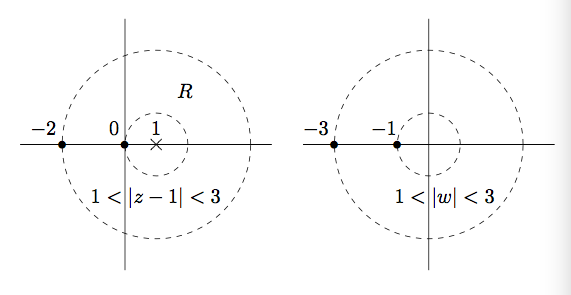
\includegraphics [scale=0.5] {writeseries1.png} \end{center}

The first thing to do is make a substitution that translates the region so that it becomes centered on the origin:  $w = z - 1$.  Then the function becomes
\[  \frac{1}{(w + 1)(w + 3)} \]
The next thing is to write partial fractions.  For the numerator we get
\[ A(w+3) + B(w+1) = 1 \]
\[ A = - B = \frac{1}{2} \]
Hence
\[ \frac{1}{2} \cdot \ [ \ \frac{1}{w+1} - \frac{1}{w+3} \ ] \]
The third step is to convert each of these fractions into something like $1/1-x$.
\[ \frac{1}{w+1} = \frac{1}{1 - (-w)} \]
\[ \frac{1}{w+3}  = \frac{1}{3} \cdot \frac{1}{1 - (-w/3)} \]
And then the fourth step is to write the series, recalling that we want different forms depending on whether we are in a circle or an annulus.

\[ \frac{1}{1 - (-w)} \]
\[ = \sum_{n=0}^{\infty} (-w)^n = \sum_{n=0}^{\infty} (-1)^n (w)^n , \ \ \ |w| < 1 \]
\[ = -\sum_{n=1}^{\infty} \frac{1}{(-w)^n} =  -\sum_{n=1}^{\infty} \frac{(-1)^n}{w^n}, \ \ \ |w| > 1 \]
We pick the second form because our region is $1 < |z-1| < 3$

A similar thing can be done for the other term.  We show only the first series since we are inside the circle.
\[  \frac{1}{3} \cdot \frac{1}{1 - (-w/3)} \]
\[ = \frac{1}{3} \cdot  \sum_{n=0}^{\infty} (-1)^n (\frac{w}{3})^n , \ \ \ |w| < 3 \]
\[ = \sum_{n=0}^{\infty} (-1)^n \ \frac{1}{3^{n+1}} \ w^n , \ \ \ |w| < 3 \]

Add the two series together (remembering the minus sign on the second term)
\[ -\sum_{n=1}^{\infty} \frac{(-1)^n}{w^n} - \sum_{n=0}^{\infty} (-1)^n \ \frac{1}{3^{n+1}} \ w^n \]
and then picking up the leading factor from 
\[ \frac{1}{2} \cdot \ [ \ \frac{1}{w+1} - \frac{1}{w+3} \ ] \]
so
\[ \frac{1}{2} \ [ \ -\sum_{n=1}^{\infty} \frac{(-1)^n}{w^n} - \sum_{n=0}^{\infty} (-1)^n \ \frac{1}{3^{n+1}} \ w^n \ ] \]

The last step is to reverse the substitution:  $w = z - 1$ and bring the minus sign out front
\[ f(z) = - \frac{1}{2} \ [ \ \sum_{n=1}^{\infty} \frac{(-1)^n}{(z-1)^n} \sum_{n=0}^{\infty} (-1)^n \ \frac{1}{3^{n+1}} \ (z-1)^n \ ] \]

I don't know if I could ever learn to do this well, but at least the explanations make sense.

Now, if we were to integrate $f(z)$, we would have only one term that gives a non-zero result, namely the first term with $n=1$
\[ - \frac{1}{2} (-1) \frac{1}{z-1} \]
\[ \text{Res }(1) = \lim_{z \rightarrow 1} \frac{1}{2} = \frac{1}{2} \]
Multiply by $2 \pi i$ to obtain $\pi i$.

\end{document}  